\documentclass[12pt]{article}
\usepackage[a4paper, total={7in,10in}]{geometry}

\usepackage{polyglossia}
\usepackage{ragged2e}
\usepackage{amsmath}
\usepackage{amssymb}
\usepackage{microtype}
\usepackage{graphicx}
\usepackage{changepage}
\usepackage{hyperref}
\usepackage{cancel}
\usepackage{wrapfig}
\usepackage{needspace}

\let\ORIincludegraphics\includegraphics
\renewcommand{\includegraphics}[2][]{\ORIincludegraphics[scale=0.65,#1]{#2}}

\graphicspath{{./images/}}
\setmainlanguage{russian}
\setotherlanguage{english}
\newfontfamily\russianfont[Script=Cyrillic]{Times New Roman}
\newfontfamily\englishfont{Times New Roman}
\setlength{\parindent}{0em}
\setlength{\parskip}{6pt}

\def\posl#1#2{\{#1_{#2}\}}
\DeclareMathOperator*{\sh-like}{\sinh-like}
\DeclareMathOperator*{\ch-like}{\cosh-like}
\DeclareMathOperator*{\th-like}{\tanh-like}
\DeclareMathOperator*{\cth-like}{\coth-like}
\DeclareMathOperator*{\tg-like}{\tan-like}
\DeclareMathOperator*{\ctg-like}{\cot-like}
\DeclareMathOperator*{\arctg-like}{\arctan-like}
\DeclareMathOperator*{\arcctg-like}{\arctan-like}

\setcounter{section}{7}

\begin{document}
    \justifying
    \begin{titlepage}
        \begin{center}
            \hfill \break
            \large{МИНОБРНАУКИ РОССИИ}\\
            \footnotesize{ФЕДЕРАЛЬНОЕ ГОСУДАРСТВЕННОЕ АВТОНОМНОЕ ОБРАЗОВАТЕЛЬНОЕ УЧРЕЖДЕНИЕ}\\ 
            \footnotesize{ВЫСШЕГО ПРОФЕССИОНАЛЬНОГО ОБРАЗОВАНИЯ}\\
            \small{\textbf{«Дальневосточный федеральный университет»}}\\
            \hfill \break
            \normalsize{ИНСТИТУТ МАТЕМАТИКИ И КОМПЬЮТЕРНЫХ ТЕХНОЛОГИЙ}\\
             \hfill \break
            \normalsize{Департамент программной инженерии и искусственного интеллекта}\\
            \hfill\break
            \hfill \break
            \hfill \break
            \hfill \break
            \large{Лекции 2 курса по дисциплине}\\
            \large{Математический Анализ}\\
            \hfill \break
            \hfill \break
            \hfill \break
            \begin{flushright}
              Подготовлено студентами гр.\\
              Б9123-02.03.03тп\\
              Макевкин C.C.\\
              Тарасенко Т.В.\\
              \hfill \break
            \end{flushright}
            \begin{center}
                Для\\
              Зиновьева Павла Владимировича
            \end{center}
            \hfill \break
            
            \hfill \break
            
            \hfill \break
            \hfill \break
            \end{center}
             
            \hfill \break
             
            \normalsize{ 
            
            }
            \begin{center} Владивосток \\ 2025 \end{center}
            \thispagestyle{empty}
    \end{titlepage}
    \pagebreak
    \tableofcontents
    \pagebreak
  \section{Криволинейные, кратные и поверхностные интегралы}
  \subsection{Криволинейные интегралы I рода}
  \underline{Определение: } Кривая $\overline{r}(t)=x(t)\overline{i}+y(t)\overline{j}$
  $a \leq t \leq b$ называется непрерывной гладкой кривой, если x(t),y(t),z(t) непрерывно дифференцируемы
  на [a;b] и $x'(t)^2+y'(t)^2+z'(t)^2 \not = 0$\\
  \underline{Определение: } Кривая называется непрерывной кусочно-гладкой кривой, если она состроит из конечного числа
  гладких кривых.\\
  Рассмотрим непрервную кусочно-гладкую кривую:\\
  \begin{minipage}{0.45\textwidth} % Левая колонка — для изображения
      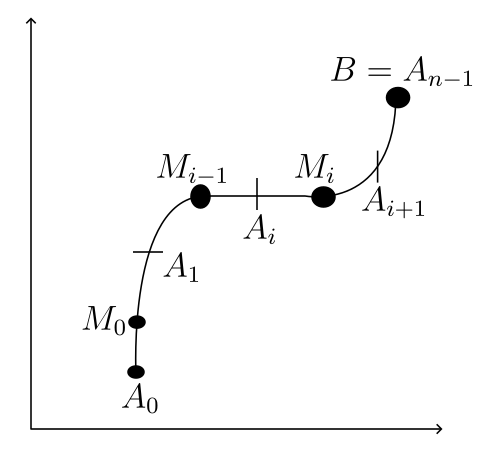
\includegraphics[width=\linewidth]{8.1.1.png}
  \end{minipage}%
  \hspace{1em} % Горизонтальный отступ между колонками
  \begin{minipage}{0.65\textwidth} % Правая колонка — для текста
      Пусть кривая имеет массу $\rho=\frac{\mathrm{kg}}{\mathrm{m}}$.
      \begin{enumerate}
        \item R
        \item В каждой элементарной $\Delta l_i$ выберем\\ произвольюную $M_i$ 
        \item Вычислим $\rho(M_i)$
        \item Считаем, что на всём $\Delta l_i \rho=const=\rho(M_i)$
        \item Составим $\sigma_R=\sum_{i=0}^{n-1}\rho(M_i)\Delta l_i$
        \item $\lim_{\lambda_R \to 0} \sigma_R = m = \int_{(l)} g dl$
      \end{enumerate}
  \end{minipage}
  \vspace{1em}
  \par Рассмотрим функцию Z=f(x,y), заданную вдоль непрервывной кусочно-гладкой кривой l\\

  \begin{minipage}{0.45\textwidth}
    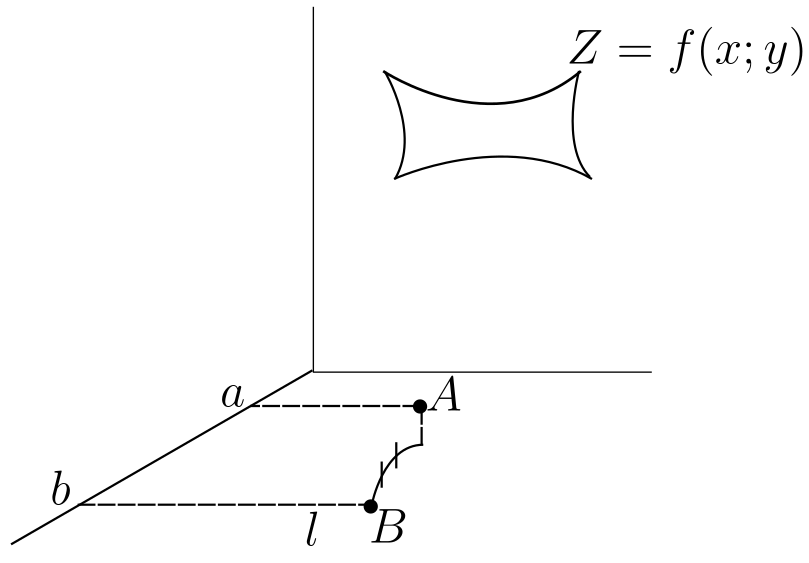
\includegraphics[scale=0.6]{8.1.2.png}
  \end{minipage}
  \hspace{1em} % Горизонтальный отступ между колонками
  \begin{minipage}{0.65\textwidth} % Правая колонка — для текста
      Пусть кривая имеет массу $\rho=\frac{\mathrm{kg}}{\mathrm{m}}$.
      \begin{enumerate}
        \item R
        \item Выберем произвольюную (.) $M_i \in \Delta l_i$\\ (.)$M_i (\xi_i;\eta_i)$
        \item Вычислим $f(\xi_i;\eta_i)$
        \item Составим $\sigma_R = \sum_{i=0}^{n-1} f(\xi_i,\eta_i) \Delta l_i$
        \item Вычислим $\lim_{\lambda_R \to 0} \sigma_R = \int_{(l)} f(x;y) dl$
      \end{enumerate}
  \end{minipage}
  \vspace{1em}
  \par
  \underline{Определение: } Если существует конечный предел интегральной суммы $\sigma_R$, не 
  зависящей от способа разбиения кривой и выбора $(.) M_i(\xi_i,\eta_i)$, то он называется
  криволинейным интегралом I рода от функции f(x;y) по кривой l.\\
  \[m=\int_{(l)} f(x;y) dl\]\\
  \underline{Замечание:} Если кривая (AB) не замкнута: \[\int_{(AB)} f(x;y)dl = \int_{(BA)} f(x;y)dl\]
  !!! При переходе к определенному интегралу пределы интегрирования ставятся по мере возрастания
  переменной интегрирования.

  \begin{minipage}{0.45\textwidth}
    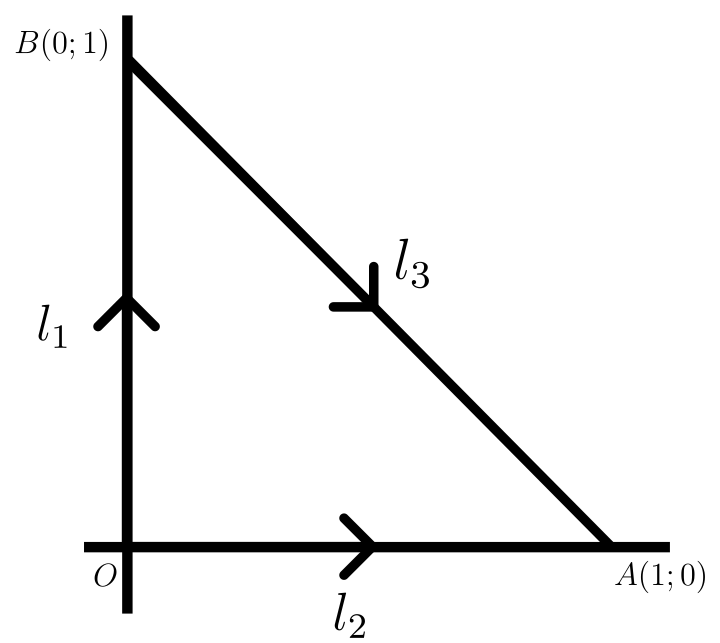
\includegraphics[scale=0.6]{8.1.3.png}
  \end{minipage}
  \hspace{1em}
  \begin{minipage}{0.65\textwidth}
      \[\int = \int_{(l_1)}+\int_{(l_2)}+\int_{(l_3)}\]\\
      \[\int_{0}^{1}\dots dy+\int_{0}^{1}\dots dx+\int_{0}^{1}\dots dx\]
  \end{minipage}
  \vspace{1em}
  \par
  \underline{Замечание:} Аналогично вводится интеграл по пространственной кривой $\int_{(l)} f(x;y;z)dl$
  \subsection{Вычисление криволинейного интеграла I рода.}
  \[\int_{(l)} f(x;y) dl \hspace{10pt} l: \begin{cases}
    x=x(t) & a\leq t\leq b\\
    y=y(t)
  \end{cases}\] \\
  \begin{minipage}{0.45\textwidth}
    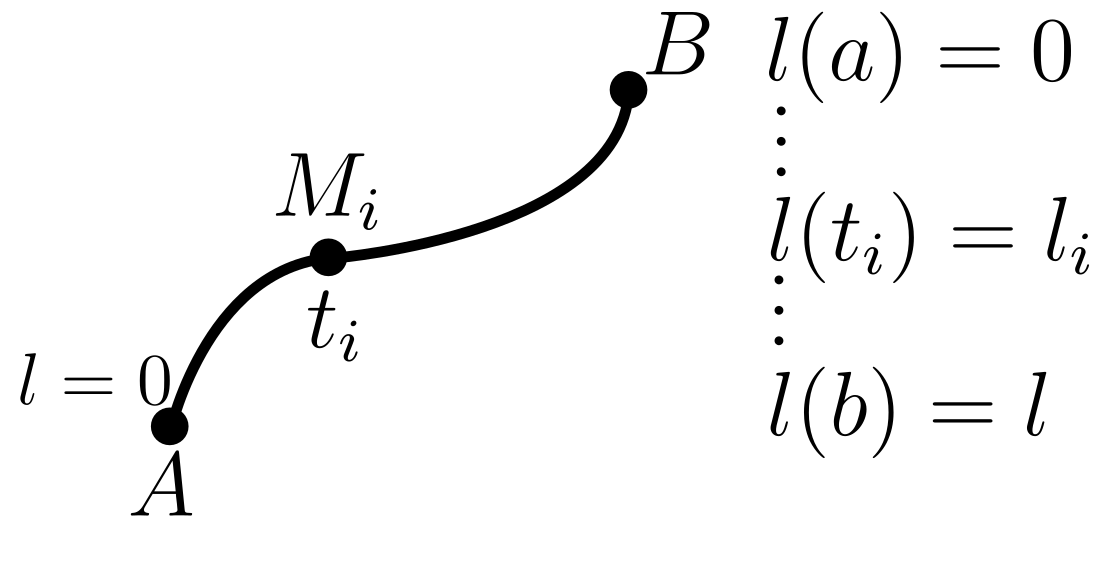
\includegraphics[scale=0.4]{8.2.1.png}
  \end{minipage}
  \hspace{1em}
  \begin{minipage}{0.65\textwidth}
    Положение (.) $M_i$ однозначно определяется с помощью \\
    длины дуги, отсчитываемой от (.)A. $\begin{cases}
      x=x(l)\\
      y=y(l)
    \end{cases}$
  \end{minipage}
  \vspace{1em}
  \par
  \[\int_{(l)}f(x;y)dl=\int_{0}^{l} f(x(l);y(l))dl\]
  \begin{enumerate}
    \item Если кривая задана уравнением y=f(x) $a \leq x \leq b$\\
    \[\int_{(l)} g(x;y)dl = \int_{a}^{b} f(x) \underbrace{\sqrt{1+f'(x)^2}dx}_{dl}\]
    \item Если кривая задана параметрически\\
    \[\begin{cases}
      x=x(t)\\
      y=y(t)
    \end{cases} t_1 \leq t \leq t_2 \hspace{20pt} \int_{(l)}g(x;y)dl=\int_{t_1}^{t_2}g(x(t);y(t))
    \sqrt{x'(t)^2+y'(t)^2}dt\]
    \item Если кривая задана $r=r(\phi) \hspace{20pt} \alpha \leq \varphi \leq \beta$\\
    \[\int_{(l)}g(x;y)dl = \int_{\alpha}^{\beta} g(r(\varphi)\cos(\varphi);r(\varphi)\sin(\varphi))
    \sqrt{r^2(\varphi)+r'(\varphi)^2}d\varphi\]
  \end{enumerate}
  \subsection*{Свойства криволинейных интегралов I-рода:}
  \begin{enumerate}
    \item $\int_{(l)}dl=L$
    \item m=$\int_{(l)}\rho dl$
    \item $x_c=\frac{M_y}{m}=\frac{\int_{(l)}\rho xdl}{\int_{(l)}\rho dl}$ \hspace{20pt}
    $M_y$ - статический момент кривой относительность оси y.\\
    $y_c = \frac{M_x}{m}=\frac{\int_{(l)}\rho ydl}{\int_{(l)}\rho dl}$ \hspace{20pt}
    $M_x$ - статический момент кривой относительно оси X
  \end{enumerate}
  \subsection{Криволинейные интегралы II рода}
  Пусть задана Z=f(x;y), которая опрелена в каждой (.) l\\
  \begin{minipage}{0.45\textwidth}
    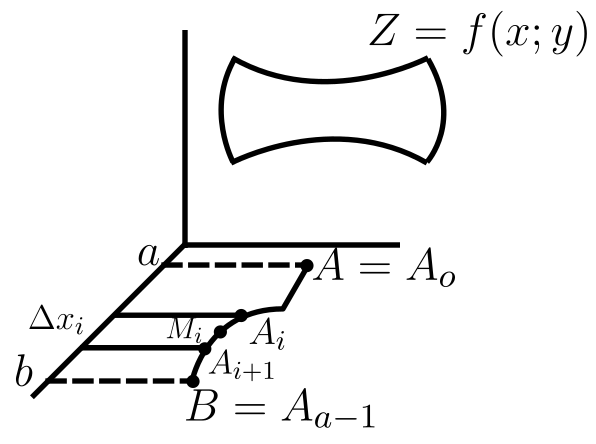
\includegraphics[scale=0.8]{8.3.1.png}
  \end{minipage}
  \hspace{1em}
  \begin{minipage}{0.65\textwidth}
    \begin{enumerate}
      \item R
      \item $M_i(\xi_i,\eta_i) \in \Delta l_i$
      \item $f(M_i)=f(\xi_i;\eta_i)$
      \item $\sum_{i=0}^{n-1}f(\xi_i;\eta_i)\Delta x_i=\sigma_R$
      \item $\lim_{\lambda_R \to 0}\sigma_R=\int_{(l)}f(x;y)dx$
    \end{enumerate}
  \end{minipage}
  \vspace{1em}
  \par
  \underline{Определение: } Если существует конечный предел суммы $\sigma_R$, не зависящей от способа
  разбиения кривой l и выбора (.) $M_i(\xi_i;\eta_i)$, то он называется криволинейным интегралом
  II рода от функции f(x;y) по кривой l\\
  \underline{Замечание:} Аналогично вводится\\
  \[\int_{(l)}f(x;y)dy\]\\
  Если вдоль кривой определенны функции $P(x;y),Q(x;y)$ и существует $\int_{(AB)}P(x;y)dx$ и
  $\int_{(AB)}Q(x;y)dy$, то $\int_{(AB)}P(x;y)dx+Q(x;y)dy$ называется криволинейным интегралом
  II рода общего вида.\\
  \underline{Замечание:} \[\int_{(AB)}f(x;y)dx=-\int_{(BA)}f(x;y)dx\]\\
  Аналогично вводится: \[\int_{(AB)}P(x;y;z)dx+Q(x;y;z)dy+R(x;y;z)dz\]
  \subsection{Существование и вычисление криволинейного интеграла II рода}
  \subsubsection*{Теорема 8.4.1}\label{th:8.4.1}
  \par\noindent
  Пусть кривая AB задана параметрически:\\
  $\begin{cases}
    x=\varphi(t) \hspace{20pt} \varphi(t),\psi(t) \text{ непрерывны } \forall t \in [a;b]\\
    y=\psi(t)
  \end{cases}$\\
  Пусть f=f(x;y) непрерывна вдоль кривой AB. $\varphi'(t)$ существует и непрерывна $\forall t \in [a;b]$.
  Тогда существует криволинейный интеграл $\int_{(AB)}f(x;y)dx=\int_{a}^{b}f(\varphi(t);\psi(t))\varphi'(t)dt$\\
  \underline{Доказательство:}
  \begin{adjustwidth}{1.5em}{1.5em}
    \begin{minipage}{0.45\textwidth}
      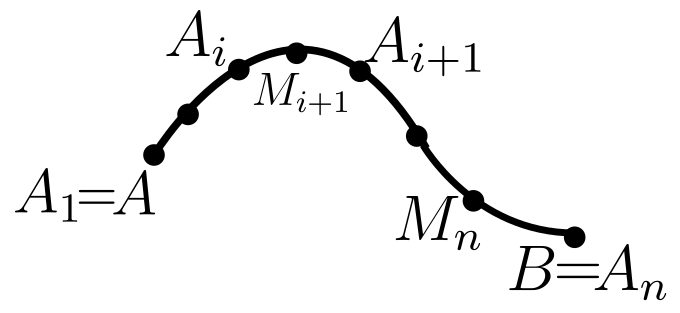
\includegraphics[scale=0.6]{8.4.1.png}
    \end{minipage}
    \hspace{1em}
    \begin{minipage}{0.55\textwidth}
      \begin{enumerate}
        \item Произведем разбиение R кривой (AB) точками $A_i(\varphi(t_i);\psi(t_i))$
        \item Выберем (.) $M_i(\varphi(\tau_i);\psi(\tau_i))$
        \item $\Delta x_i = \varphi(t_{i+1})-\varphi(t_i)=\int_{t_i}^{t_{i+1}}\varphi'(t)dt$
        \item $\sigma_R=\sum_{i=0}^{n-1}f(\varphi(\tau_i);\psi(\tau_i))\Delta x_i=\\=\sum_{i=0}^{n-1}
        f(\varphi(\tau_i);\psi(\tau_i))\int_{t_i}^{t_{i+1}}\varphi'(t)dt$
      \end{enumerate}
    \end{minipage}
    \vspace{1em}
    \par
  \end{adjustwidth}
  Рассмотрим правую часть: $\int f(\varphi(\tau_i);\psi(\tau_i))\varphi'(t)dt = \sum_{i=1}^{n}
    \int_{t_i}^{t_{i+1}}f(\varphi(\tau_i);\psi(\tau_i))\varphi'(t)dt=I$\\
  Рассмотрим $|\sigma_R-I|=\sum_{i=1}^{n} \int_{t_i}^{t_{i+1}} [f(\varphi(\tau_i);\psi(\tau_i))-
  f(\varphi(t);\psi(t))]\varphi'(t)dt \boxed{<}$\\
  Т.к. f(x;y) непрерывна вдоль кривой (AB)\\
  \[\forall \varepsilon >0 \exists \delta = \delta(\varepsilon):|\Delta t_i| < \delta \Rightarrow
  |f(\varphi(t_{i+1});\psi(t_{i+1}))-f(\varphi(t_i);\psi(t_i))|<\varepsilon\]\\
  или $\begin{matrix}
    [t_i;\tau_i] <[t_i;t_{i+1}]\\
    [\tau_i;t_{i+1}] < [t_i;t_{i+1}]
  \end{matrix} \hspace{20pt} \varphi'(t)$ непрерывна на $[t_i;t_{i+1}] \Rightarrow$ она ограничена на нём.\\
  Пусть $\forall i |\varphi'(t_i)|<L$\\
  \boxed{<} $|\varepsilon L \sum_{i=1}^{n} \int_{t_i}^{t_{i+1}}dt|=\varepsilon L(b-a)\Rightarrow \lim_{\lambda_R \to 0}\sigma_R=I$
  \begin{center}
    \textbf{Ч.т.д.}
  \end{center}
  Аналогично: \[\int_{(AB)}f(x;y)dy=\int_{a}^{b}f(\varphi(t);\psi(t))\psi'(t)dt\]\\
  Если кривая задана как y=y(x) \hspace{10pt} $a\leq x\leq b$. Тогда\\
  $\begin{cases}
    y=y(t)\\
    x=t
  \end{cases} \hspace{20pt} a\leq t\leq b \Rightarrow \int_{(AB)}f(x;y)dx =\int_{a}^{b} f(t;y(t))dt=
  |x=t|=\int_{a}^{b}f(x;y(x))dx$\\
  \underline{Замечание:} $\int_{(AB)}f(x;y)dx=0,$ если AB-прямоугольный отрезок || оси OY. Аналогично \\
  $\int_{(CD)}f(x;y)dy=0,$ если CD-прямоугольный отрезок || OX.\\
  Если L-замкнутый контур.\\
  \begin{minipage}{0.45\textwidth}
    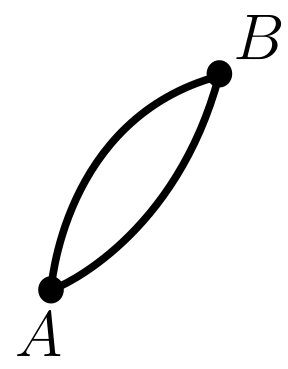
\includegraphics[scale=0.6]{8.4.2.png}
  \end{minipage}
  \hspace{1em}
  \begin{minipage}{0.25\textwidth}
    \[\int_{(l)}=\int_{(AB)}+\int_{(BA)}\]
  \end{minipage}
  \vspace{1em}
  \par
  Среди двух возможных обходов, L обход против часовой стрелки, причём за положительный обход. При обходе рассматриваемая область
  находится слева.
  \subsection{Вычисление площади криволинейной трапеции с помощью криволинейного интеграла.}
  \begin{minipage}{0.45\textwidth}
    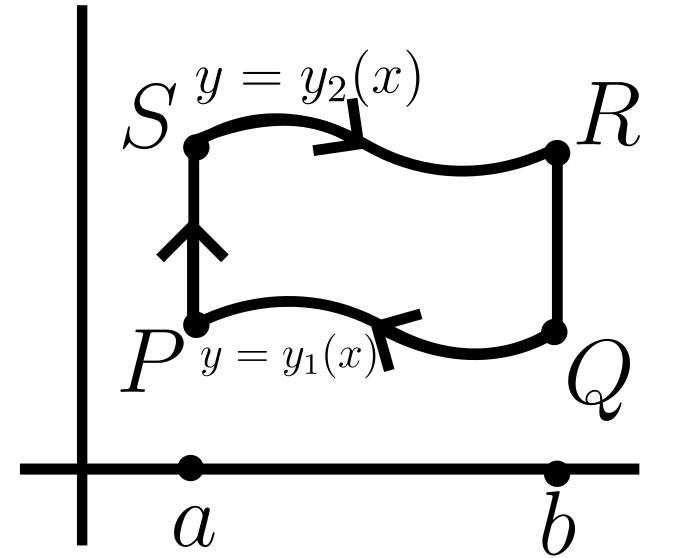
\includegraphics[scale=0.6]{8.5.1.png}
  \end{minipage}
  \hspace{1em}
  \begin{minipage}{0.55\textwidth}
    Найти S(PSRQ)\\
    \[S=\int_{a}^{b}y_2(x)dx-\int_{a}^{b}y_1(x)dx \boxed{=}\]\\
     \[\text{Рассмотрим} \int_{a}^{b}y_2(x)dx=\int_{(SR)}ydx\]\\
      \[\text{Рассмотрим}\int_{a}^{b}y_1(x)dx=\int_{(PQ)}ydx\]\\
    $\boxed{=} \int_{(SR)}ydx-\int_{(PQ)}ydx=\int_{(SR)}ydx+\int_{(QP)}ydx+$ \\ 
    \par
    $\int_{(PS)}ydx+\int_{(RQ)}ydx=\int_{(PSRQP)}ydx \boxed{=}$
  \end{minipage}
  \vspace{1em}
  \par
  Пусть L=(PQRSP) - контур взятый в положительном направлении. $\boxed{=}-\int_{(L)}ydx=S$\\
  Аналогично, если рассмотреть:
  \begin{flushleft}
    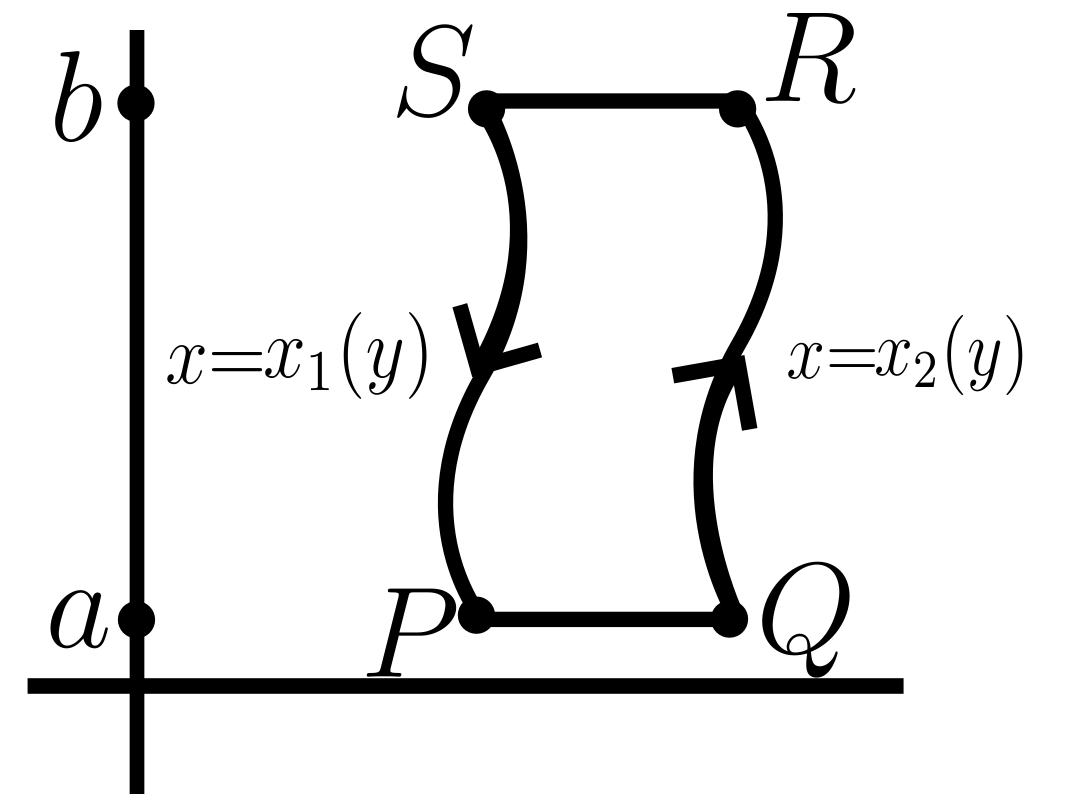
\includegraphics[scale=0.4]{8.5.2.png}
  \end{flushleft}
  То получим S=$\int_{(l)}xdy$\\
  Для произвольного замкнутого контура L\\
  \[\boxed{S=\frac{1}{2}\int_{(l)}xdy-ydx}\]
  \underline{Замечание:}
  \begin{flushleft}
      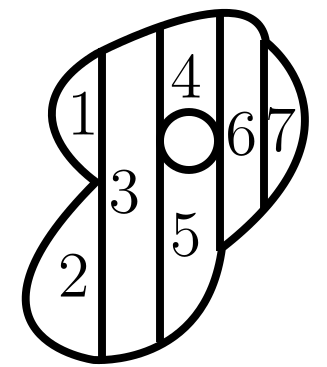
\includegraphics{8.5.3.png}
  \end{flushleft}
  \subsection{Связь медлу криволинейными интегралами I и II рода}
\end{document}